\section{Software Architecture: Service Decomposition}

%%Texto introductorio


%%%%% DE AQUÍ EN ADELANTE
%%%%% Subsubsection por frente
\subsection{Architectural Style}

%%% Definición de cada frente
%%% Aquí agreguen diagrama de arquitectura de su frente 
%%%

% ------------------------- Payments and Refunds -------------------------
\begingroup
\setlength{\emergencystretch}{3em}
\subsubsection{Payments and Refunds}
\label{sec:pay-style}

This work stream covers every money movement of the platform: the payment
inside \emph{Book Accommodation}, the refunds caused by \emph{Cancel
Reservation}, the manual refunds of \emph{Handle Refunds} (Customer Support)
and the payouts to hosts. The payment gateway is an \textbf{external system}:
it moves the money and processes card data. The architecture only
\emph{orchestrates} the gateway, records what was requested and answered, and
keeps the accounts of who owns each part of the money. Card numbers never
enter the system; clients tokenize the card directly with the gateway and the
platform only stores the token.

\paragraph{Requirements gap.} The Delivery~1 catalogue (FR01--FR10) has no
functional requirement for payments, although three use cases depend on them.
We propose two additions: \textbf{FR11}, \emph{the system shall orchestrate
the guest payment of a reservation through the external gateway and shall
never charge a guest twice for the same reservation}; and \textbf{FR12},
\emph{the system shall issue full or partial refunds and shall record every
charge, refund and payout in an auditable ledger that separates the platform
margin from the amount owed to the host}.

\paragraph{Services.} The work stream is split into two services. The name
\emph{Payment Coordination} is the one already used by the Reservation work
stream.

\begin{longtable}{@{}L{3.0cm}L{10.8cm}@{}}
\toprule
\textbf{Service} & \textbf{Responsibility} \\
\midrule
\endhead
\textbf{Payment Coordination Service} &
  Creates the payment of each reservation, asks the gateway to authorize,
  capture, void and refund, receives the gateway webhooks, and guarantees
  that a guest is never charged twice. It does \emph{not} compute prices,
  decide refund amounts or keep balances. \\
\addlinespace
\textbf{Ledger \& Payout Service} &
  Double-entry, append-only ledger that splits every charge between the host
  and the platform margin, schedules host payouts, asks the gateway to pay
  hosts, and serves balances and reports to support agents and auditors. It
  never talks to the guest's payment method. \\
\bottomrule
\caption{Services of the Payments and Refunds work stream.}
\label{tab:pay-services}
\end{longtable}

\paragraph{Why two services and not one.} Gateway integration changes often,
while accounting rules must stay stable and auditable. Keeping the ledger
separate means a slow or failing ledger never blocks a guest's payment, and
the ledger can stay append-only.

\paragraph{Payment states.}
\begin{longtable}{@{}L{4.2cm}L{9.6cm}@{}}
\toprule
\textbf{State} & \textbf{Meaning} \\
\midrule
\endhead
\texttt{AUTHORIZED} & The money is held on the guest's card, not charged yet. \\
\texttt{PENDING} & Waiting for the bank (3-D Secure, slow method), or the gateway did not answer in time. \\
\texttt{DECLINED} & The bank rejected the attempt; the guest may try another method. \\
\texttt{FAILED} & Attempts exhausted, or the reservation expired before a result. \\
\texttt{CAPTURED} & The money was charged (point of no return). \\
\texttt{VOIDED} & The hold was released before charging. \\
\texttt{PARTIALLY\_\allowbreak REFUNDED} & Part of the charge was returned. \\
\texttt{REFUNDED} & All of the charge was returned. \\
\bottomrule
\caption{Payment states.}
\label{tab:pay-states}
\end{longtable}

\paragraph{Booking flow.} The flow follows the saga already defined by the
Reservation Service (hold of 10 minutes in \texttt{PENDING\_\allowbreak PAYMENT},
confirmation on \texttt{Payment\allowbreak Succeeded}):
\begin{enumerate}
  \item After inserting the hold, the Reservation Service calls
    \texttt{POST} \url{/api/v1/payments} with key
    \texttt{book:\allowbreak \{reservation\allowbreak Id\}:\allowbreak auth:\allowbreak \{n\}} and the frozen
    \texttt{price\_\allowbreak snapshot} of the reservation.
  \item Payment Coordination stores the payment, the attempt and the
    idempotency record \emph{before} calling the gateway, then asks it to
    \textbf{hold} the money. It waits at most about 0.8\,s, within the
    Reservation Service timeout of about 1\,s.
  \item It answers \texttt{201 AUTHORIZED}, \texttt{402 DECLINED} or
    \texttt{202 PENDING}, and publishes \texttt{Payment\allowbreak Succeeded} or
    \texttt{Payment\allowbreak Failed} through the outbox.
  \item The Reservation Service confirms the reservation and publishes
    \texttt{Reservation\allowbreak Confirmed}. Payment Coordination consumes it and
    \textbf{captures} the money, then publishes \texttt{Payment\allowbreak Captured}.
  \item The Ledger consumes \texttt{Payment\allowbreak Captured} and writes one balanced
    journal transaction (host amount and platform margin).
  \item About 24\,h after check-in (the \texttt{startDate} carried by
    \texttt{Reservation\allowbreak Confirmed}), as Airbnb does for short
    stays~\cite{airbnb-payouts}, the Ledger asks the gateway to pay the host
    and publishes \texttt{Payout\allowbreak Status\allowbreak Changed}.
\end{enumerate}

\paragraph{Declined and pending payments.}
\begin{itemize}
  \item \textbf{Declined:} no automatic retry. The guest may try another
    method on the same payment while the hold lasts; after three declined
    attempts the payment is \texttt{FAILED} and \texttt{Payment\allowbreak Failed} lets the
    Reservation Service release the dates.
  \item \textbf{Pending:} the final result arrives as a gateway webhook. A
    \emph{reconciler} runs every 5 minutes and asks the gateway, with the same
    key, about payments pending for more than 2 minutes, in case a webhook was
    lost. A timeout is \emph{never} treated as a failure, because the money may
    have moved.
  \item \textbf{Hold expired:} when the Reservation Service publishes
    \texttt{Reservation\allowbreak Expired}, Payment Coordination voids any authorization
    of that reservation, so the guest is never charged for dates they do not
    have. If the Reservation Service recovers the dates with a new hold
    (late-payment rule), it confirms and the capture happens as usual.
\end{itemize}

\paragraph{Cancellation.} The Reservation Service applies the cancellation
policy of its snapshot, cancels and calls \texttt{POST} \url{/api/v1/refunds} with
key \texttt{ref:\allowbreak \{reservation\allowbreak Id\}:\allowbreak cancel}. If the payment was not captured,
Payment Coordination voids instead of refunding. A refund rejected by the
gateway does not undo the cancellation: \texttt{Refund\allowbreak Status\allowbreak Changed}
(\texttt{FAILED}) lets the Support Service open or update a case.

\paragraph{Manual refund (Handle Refunds).} The Support Service manages the
case but does not execute refunds. The agent calls
\texttt{POST} \url{/api/v1/refunds} with the case identifier and chooses who funds
the refund. Because it is a sensitive administrative action, Payment
Coordination first appends a record to the Audit Service; if the append
cannot be confirmed, the refund is not accepted (audit before effect).

\begin{figure}[H]
  \centering
  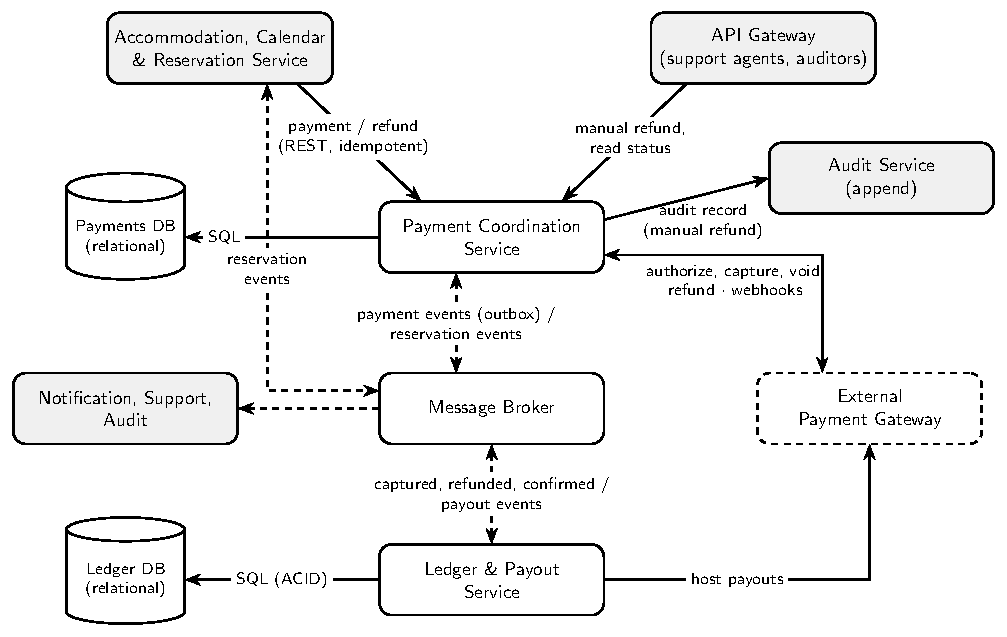
\includegraphics[width=\linewidth]{images/payments_components.pdf}
  \caption{Payments and Refunds components. Grey boxes belong to other work
  streams; the dashed box is external. Solid arrows are synchronous, dashed
  arrows are asynchronous.}
  \label{fig:pay-components}
\end{figure}
\endgroup

\subsubsection{Reservation and Calendar}
The \textbf{Reservation and Accommodation Service} is a domain-oriented
microservice that owns accommodations, the availability calendar (holds,
confirmed reservations and host blocks), reservations and check-in/check-out
agreements. It covers \emph{Book Accommodation}, \emph{Cancel Reservation},
\emph{Manage Reservations} (host), \emph{Manage Accommodation Listing} and the
administrative pause of accommodations (FR01--FR06, FR10). It uses
\textbf{synchronous commands} where the user needs an immediate answer (hold,
listing save) and \textbf{asynchronous events} for payment results,
notifications and search refresh; booking and payment form a \textbf{saga}, not
a distributed transaction. When a host creates or edits an accommodation, the
service calls the Pricing Service with guest capacity, base price and cleaning
flag and stores the returned multiplier. Workload: booking and payment are
5\,\% of traffic ($\approx 13$ req/s average and $\approx 130$ req/s at peak at
real scale; 25 and 60 req/h in the simulation).

\begin{figure}[H]
\centering
\begin{tikzpicture}[
  scale=0.72, transform shape,
  font=\sffamily\small,
  >={Stealth[length=2.5mm]},
  svc/.style={draw, thick, rounded corners=6pt, minimum width=3.6cm,
              minimum height=1.2cm, align=center, fill=white},
  oth/.style={svc, fill=gray!12},
  ext/.style={svc, dashed},
  db/.style={cylinder, shape border rotate=90, draw, thick, aspect=0.25,
             minimum width=1.9cm, minimum height=1.8cm, align=center, fill=white,
             font=\sffamily\footnotesize},
  flow/.style={->, dashed, thick},
  sync/.style={->, thick},
  lbl/.style={fill=white, inner sep=2pt, align=center, font=\sffamily\footnotesize}
]
  \node[oth] (apigw) at (0, 5.5)  {API Gateway};
  \node[svc] (res)   at (0, 1.5)  {Reservation and\\Accommodation Service\\(listings, calendar,\\reservations)};
  \node[db]  (resdb) at (0,-2.8)  {Service DB\\(PostgreSQL)};
  \node[oth] (price) at (-6, 1.5) {Pricing\\Service};
  \node[oth] (pay)   at (6, 1.5)  {Payment\\Coordination};
  \node[ext] (gate)  at (6,-2.8)  {External\\Payment Gateway};
  \node[svc] (broker) at (6, 5.5) {Message Broker};
  \node[oth] (cons)  at (-6, 5.5) {Search, Notification,\\Support and Admin.};
  \node[svc] (timer) at (-6,-2.8) {Hold timer\\(scheduler, sweeper)};

  \draw[sync] (apigw.south) -- node[lbl]{REST} (res.north);
  \draw[sync] (res.south) -- node[lbl]{SQL\\(ACID)} (resdb.north);
  \draw[sync, <->] (res.west) -- node[lbl]{multiplier request /\\occupancy query} (price.east);
  \draw[sync] (res.east) -- node[lbl]{payment\\intent} (pay.west);
  \draw[sync, <->] (pay.south) -- node[lbl]{charge /\\refund} (gate.north);
  \draw[flow, <->] (broker.south west) -- node[lbl, pos=0.45]{reservation and\\payment events} (res.north east);
  \draw[flow] (pay.north) -- node[lbl, pos=0.55]{payment\\events} (broker.south);
  \draw[flow] (broker.north) -- ++(0,0.9) -| (cons.north);
  \node[lbl] at (0,6.4) {listing, reservation and availability events};
  \draw[flow] (timer.north) -- node[lbl, pos=0.4]{HoldExpired} (res.south west);
  \draw[flow] (timer.east) -- node[lbl, above=2pt]{expired holds} (resdb.west);
\end{tikzpicture}
\caption{Reservation and Accommodation Service. Solid arrows are synchronous
calls, dashed arrows are events; grey boxes belong to other fronts.}
\end{figure}

% ------------------------- Pricing Engine -------------------------
\begingroup
\setlength{\emergencystretch}{3em}
\subsubsection{Pricing Engine}
\label{sec:price-style}

This work stream computes the \textbf{pricing multiplier} of every
accommodation (FR03). The multiplier is applied to the host's base price to
obtain the effective nightly rate, and it is also the \textbf{platform
margin} used by Payments (Section~\ref{sec:pay-model}): it takes one of three
values, \textbf{1.02}, \textbf{1.07} or \textbf{1.15}. The Reservation and
Accommodation Service requests it \emph{synchronously} when a host creates or
edits a listing and stores it in the accommodation; it is then frozen in the
price snapshot of each reservation, so the engine never changes the price of
an existing booking.

\paragraph{How the multiplier is computed.} Each request is answered from a
\textbf{precomputed snapshot of the zone}, never by calling other services or
external APIs during the request:
\begin{itemize}
  \item \textbf{Demand indicators} (per zone, daily): \emph{occupancy rate}
    of the coming 90 days (calendar occupancy API), \emph{booking pace}
    (change of booked nights in the last 7 days) and \emph{search index}
    (searches of the zone in the last 7 days against its 4-week average,
    from the search events).
  \item \textbf{Context indicators} (per zone, monthly): local events
    (concerts, fairs, holidays) obtained from SerpAPI, an external events
    API, summarized as an impact score between 0 and 1.
  \item \textbf{Listing inputs} received in the request: maximum guests, base
    price and whether cleaning is included.
\end{itemize}
A weighted score ($0.6\cdot$demand $+\ 0.3\cdot$context $+\ 0.1\cdot$listing)
is mapped to a tier: \texttt{LOW} (1.02), \texttt{STANDARD} (1.07) or
\texttt{HIGH} (1.15). Weights and thresholds belong to a \textbf{model
version}; a new version is applied only after an administrator approves it
(human supervision), and the approval is recorded in the Audit Service. If a
zone has no snapshot yet, the engine answers \texttt{STANDARD} with
\texttt{fallback = true}, so saving a listing never fails because of missing
indicators.

\paragraph{Services.} The work stream has three services; ingestion of
indicators is separated from the request path so that search traffic and the
external API never affect the latency of a listing save.

\begin{longtable}{@{}L{3.2cm}L{10.6cm}@{}}
\toprule
\textbf{Service} & \textbf{Responsibility} \\
\midrule
\endhead
\textbf{Pricing Service} &
  \texttt{pricing-api} answers the multiplier request, stores one history
  record per calculation and manages model versions (create, approve,
  activate). \texttt{pricing-worker} applies the indicator events to the zone
  snapshot and archives history older than one year. It does \emph{not}
  store accommodations, publish prices or compute payments. \\
\addlinespace
\textbf{Demand Indicators Service} &
  Counts search events per zone and, once a day, reads the calendar
  occupancy of each zone and publishes \texttt{Demand\allowbreak Indicators\allowbreak Updated}.
  It never reads the Search or Reservation databases. \\
\addlinespace
\textbf{Context Indicators Service} &
  Monthly job that queries SerpAPI by city and month, normalizes the events
  per zone and publishes \texttt{Context\allowbreak Indicators\allowbreak Updated}. It isolates the
  only external dependency of the work stream. \\
\bottomrule
\caption{Services of the Pricing Engine work stream.}
\label{tab:price-services}
\end{longtable}

\begin{figure}[H]
  \centering
  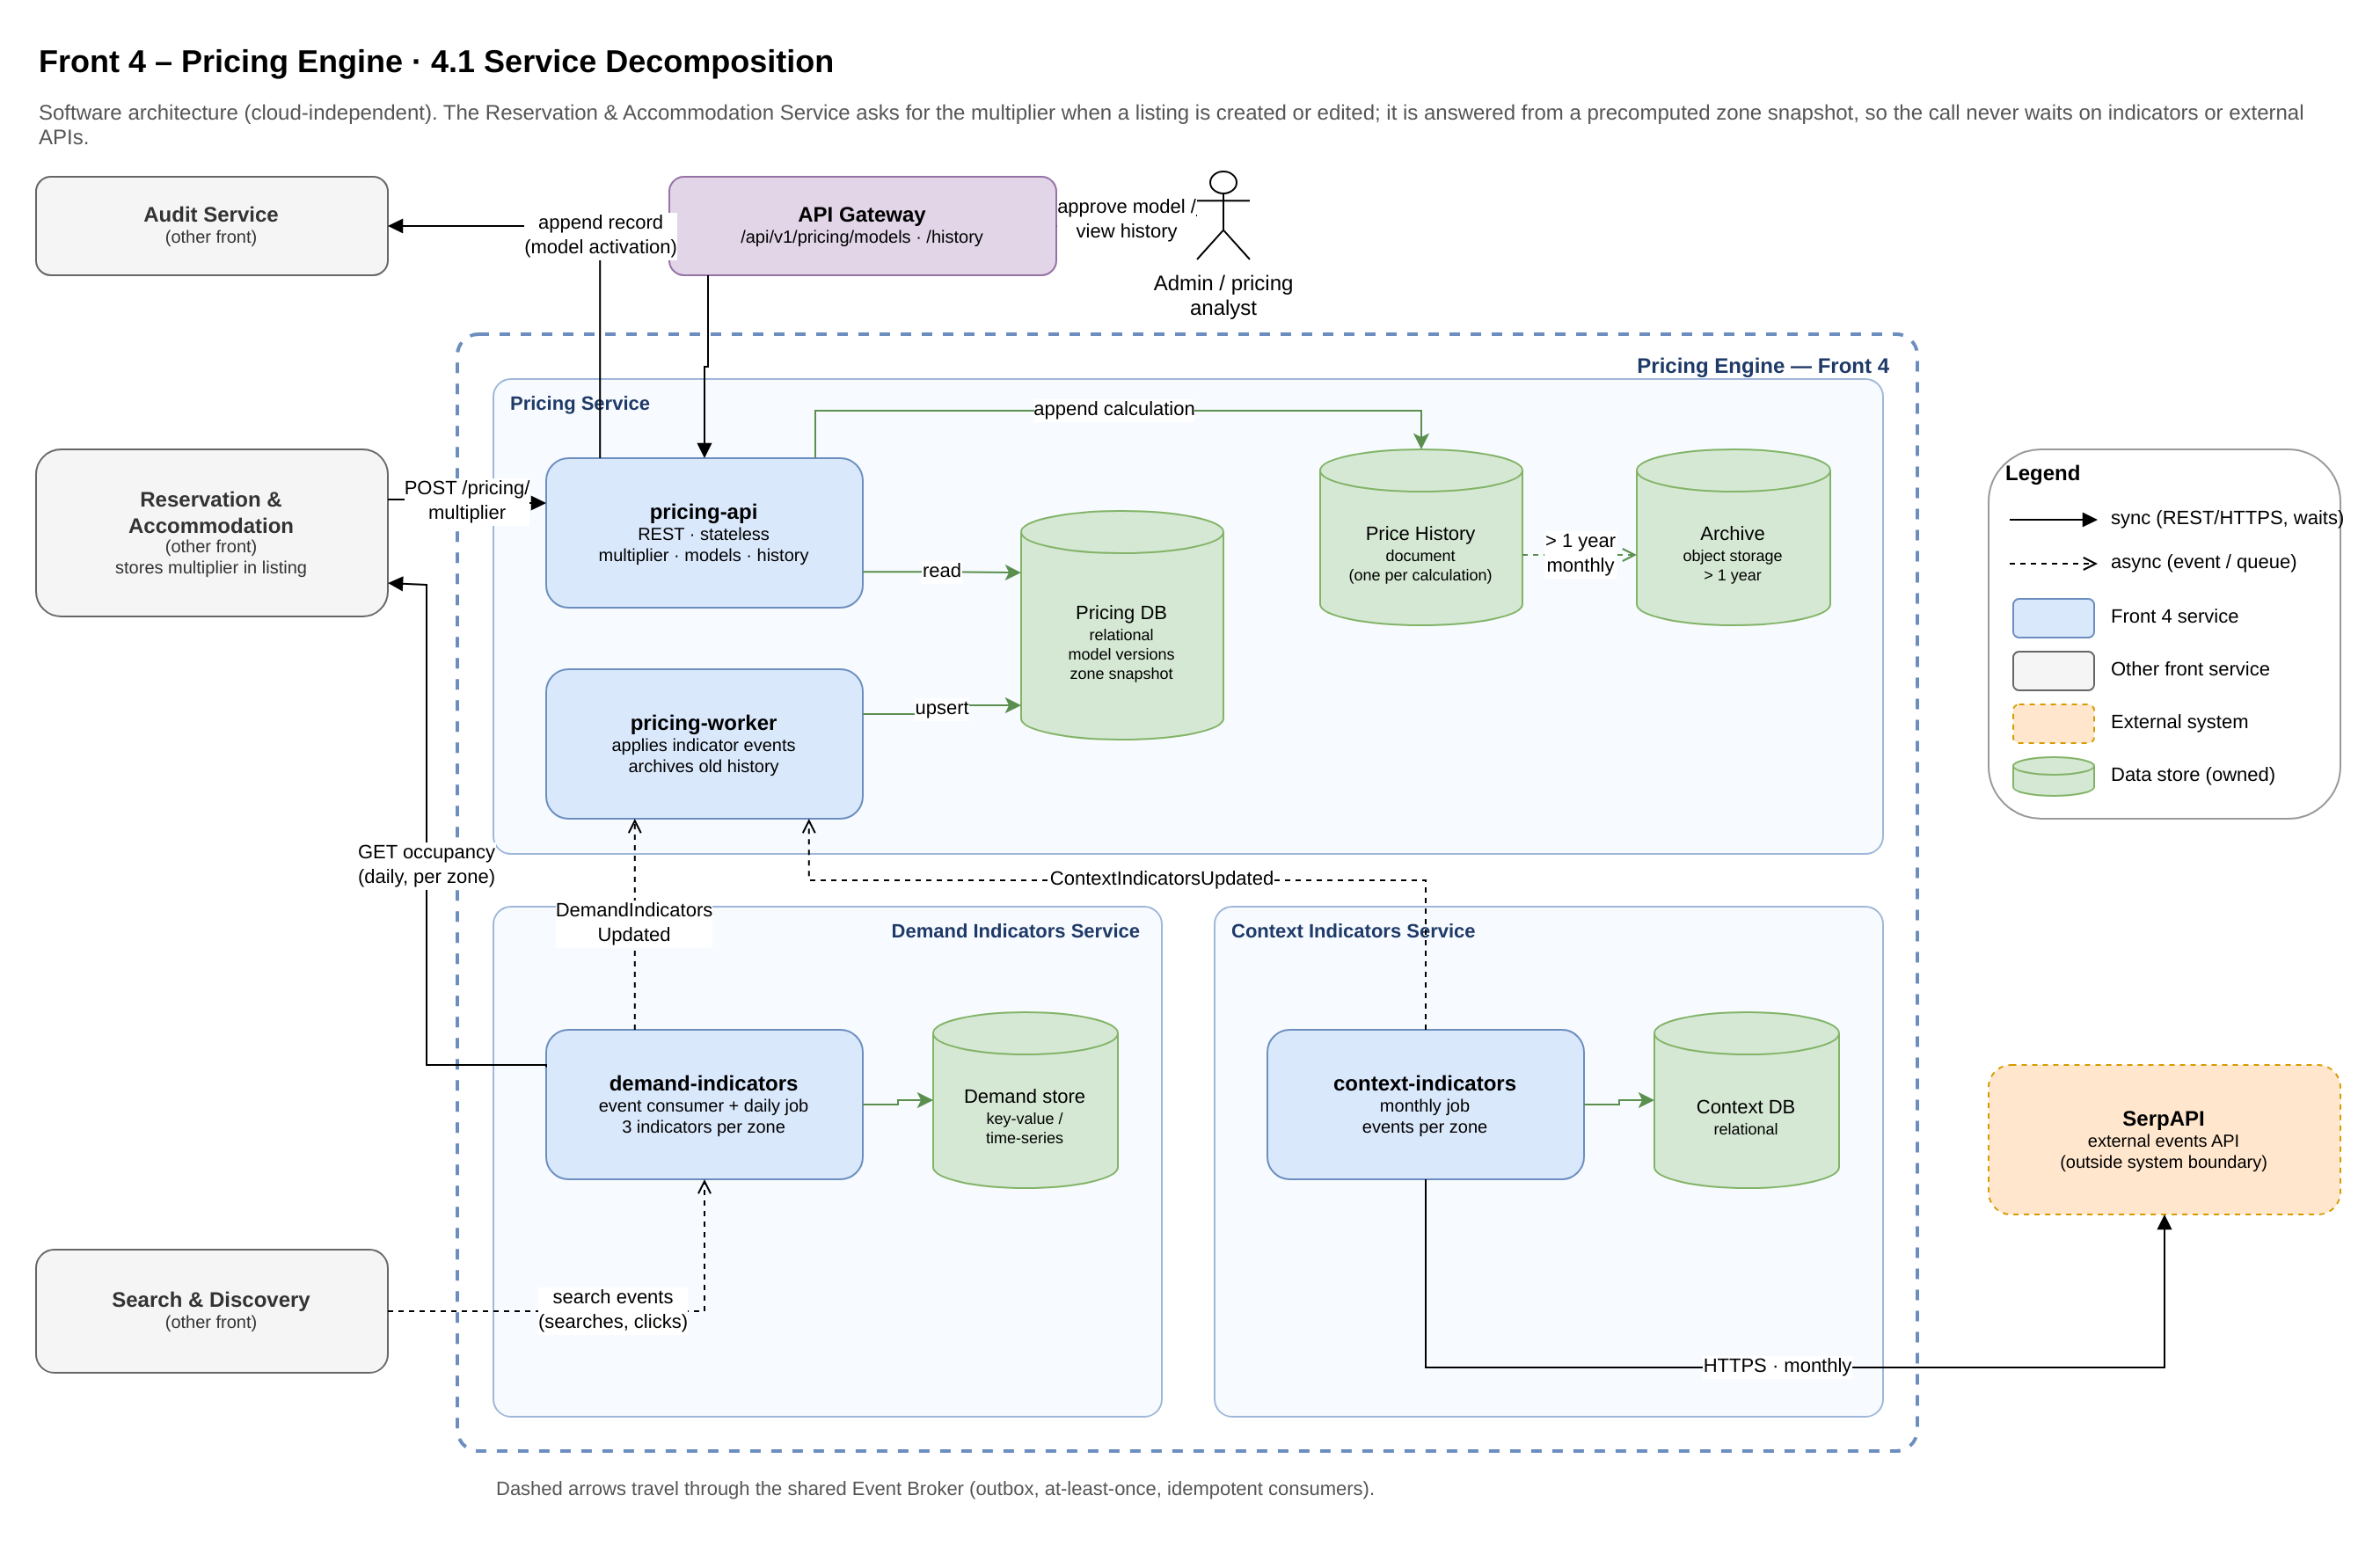
\includegraphics[width=\linewidth]{images/pricing_41_service_decomposition.png}
  \caption{Pricing Engine components. Grey boxes belong to other work streams;
  the dashed box is external. Solid arrows are synchronous, dashed arrows are
  events through the broker. Source: page 4.1 of \texttt{AirbnbCC.drawio}.}
  \label{fig:price-components}
\end{figure}
\endgroup

% ------------------------- Identity, Communication and Internal Operations -------------------------
\begingroup
\setlength{\emergencystretch}{3em}
\subsubsection{Identity, Communication and Internal Operations}
\label{sec:id-style}

This work stream covers FR09 and FR10 (authentication and role-based access
for the visitor, guest, host, administrator, auditor and support agent),
communication between guests and hosts, notifications, support cases, the
privileged administration of users and accommodations, and the immutable audit
of administrative actions. It has \textbf{seven independently deployable
services} behind the API Gateway. Three rules apply to all of them: every
service validates the token and still authorizes the specific resource (deny
by default); events are delivered at least once to idempotent consumers; and a
sensitive administrative action is confirmed only after its audit record is
appended. Visitors reach only public pages, registration and login; guests and
hosts reach only their own profile, conversations, cases and listing;
administrators, auditors and support agents are privileged roles that require
MFA, and administrators also need a fresh step-up for sensitive actions.

\begin{longtable}{@{}L{3.1cm}L{10.7cm}@{}}
\toprule
\textbf{Service} & \textbf{Responsibility} \\
\midrule
\endhead
\textbf{Identity \& Access Service} &
  Registration, login, token issuance and refresh, MFA, password reset,
  session revocation and publication of the public signing keys. It does
  \emph{not} store profile data or decide access to business resources. \\
\addlinespace
\textbf{User Profile Service} &
  Profile, contact data, role assignments and account status. It never stores
  credentials. \\
\addlinespace
\textbf{Messaging Service} &
  Conversations, message history, read state and real-time delivery. It does
  not choose channels or retry policy. \\
\addlinespace
\textbf{Notification Service} &
  Channel selection, templates, preferences, delivery attempts, retries,
  fallback and duplicate suppression. It does not own the events that trigger
  a notification. \\
\addlinespace
\textbf{Support Service} &
  Support cases: assignment, status transitions and comments. It does not
  execute refunds or change reservations or payments. \\
\addlinespace
\textbf{Administration Service} &
  Privileged workflows of Manage Users and Manage Accommodations: policy
  check, step-up MFA, reason, delegation to the owning service and audit. It
  owns no profile or accommodation data. \\
\addlinespace
\textbf{Audit Service} &
  Append-only, hash-chained audit records, integrity verification and
  read-only queries. It never updates or deletes a record. \\
\bottomrule
\caption{Services of the Identity, Communication and Internal Operations work
stream.}
\label{tab:id-services}
\end{longtable}

\paragraph{Why these boundaries.} Credentials and sessions have different
security and scaling needs from profile data, so they are separate. A message
must be stored even if every notification channel is down, so Messaging and
Notification are separate. Customer casework (Support) is not privileged
administration, and immutable evidence needs its own retention and read-only
access model (Audit). Administration only orchestrates: it delegates each
change to the service that owns the data, so there is no shared administrative
database.

\begin{figure}[H]
  \centering
  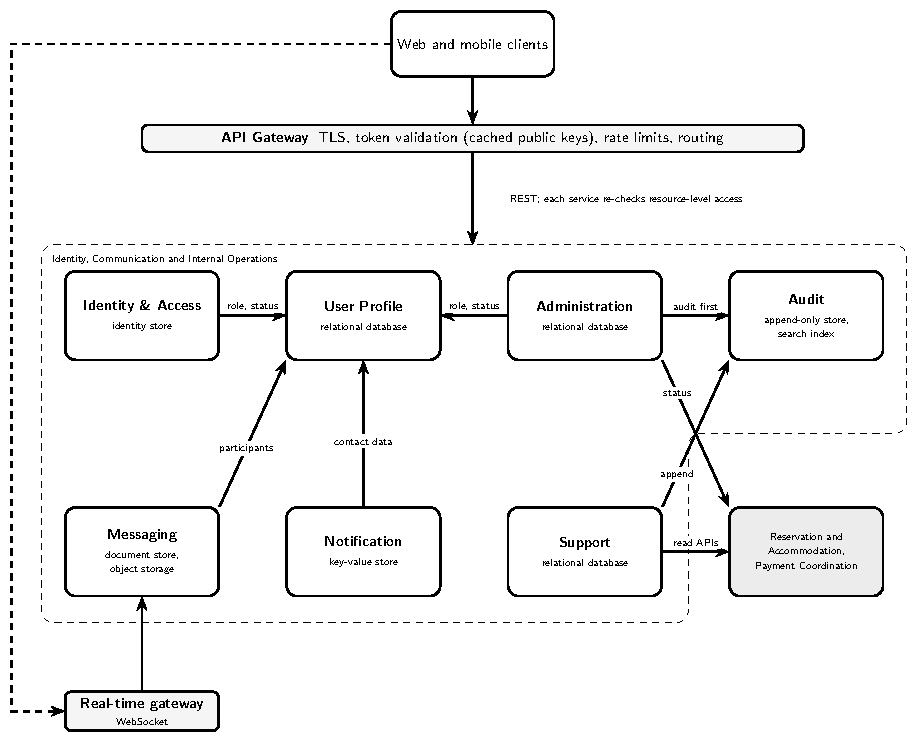
\includegraphics[width=\linewidth]{images/identity_components.pdf}
  \caption{Identity, Communication and Internal Operations components.
  Solid arrows are synchronous calls; events through the broker are shown in
  Figure~\ref{fig:id-events}. The grey box belongs to other work streams.}
  \label{fig:id-components}
\end{figure}
\endgroup

\subsection{API Contracts}
%%%
%%% AGREGUEN EN TABLITA LOS ENDPOINTS
%%% 

% ------------------------- Payments and Refunds -------------------------
\begingroup
\setlength{\emergencystretch}{3em}
\subsubsection{Payments and Refunds}
\label{sec:pay-api}

All paths are versioned under \texttt{/api/v1}. Every money-moving request
requires an \texttt{Idempotency-Key} header. Tokens are validated locally with
the keys published by Identity \& Access, and each endpoint also checks the
role and the resource (deny by default).

\begin{longtable}{@{}L{1.65cm}L{4.65cm}L{2.3cm}L{5.0cm}@{}}
\toprule
\textbf{Method} & \textbf{Endpoint} & \textbf{Caller} & \textbf{Purpose and codes} \\
\midrule
\endhead
\multicolumn{4}{@{}l}{\emph{Payment Coordination Service}} \\
POST & \url{/api/v1/payments} & Reservation Service &
  Create the payment and hold the money. Body: reservation, guest, host,
  amount, currency, price snapshot, card token. \texttt{201} authorized,
  \texttt{202} pending, \texttt{402} declined, \texttt{409} same key in
  progress, \texttt{422} same key with another body. \\
POST & \url{/api/v1/payments/{paymentId}/attempts} & Guest &
  New attempt with another method after a decline. \texttt{201},
  \texttt{202}, \texttt{402}, \texttt{409} attempts exhausted. \\
GET & \url{/api/v1/payments/{paymentId}}\newline \url{/api/v1/payments?reservationId=} &
  Guest, Support Service & Current state of a payment (read API of
  Support). \texttt{200}, \texttt{403}, \texttt{404}. \\
POST & \url{/api/v1/refunds} & Reservation Service, support agent &
  Request a refund: after a cancellation (amount from the policy), or manual
  with \texttt{supportCaseId}, \texttt{reason} and \texttt{fundedBy}.
  Processed asynchronously. \texttt{202}, \texttt{400} above refundable
  balance, \texttt{403}, \texttt{404}. \\
GET & \url{/api/v1/refunds/{refundId}} & Guest, support agent &
  State of a refund. \texttt{200}, \texttt{403}, \texttt{404}. \\
POST & \url{/api/v1/payments/webhooks/gateway} & External gateway &
  Signed notification; stored in the inbox. \texttt{200} (also duplicates),
  \texttt{401} invalid signature. \\
\addlinespace
\multicolumn{4}{@{}l}{\emph{Ledger \& Payout Service}} \\
GET & \url{/api/v1/ledger/hosts/{hostId}/balance} & Host, admin &
  Pending and released earnings. \\
GET & \url{/api/v1/ledger/hosts/{hostId}/payouts} & Host, admin &
  Payout history (\texttt{from}, \texttt{to}, \texttt{limit}). \\
GET & \url{/api/v1/ledger/reservations/{reservationId}/entries} & Support,
  auditor & Accounting entries of one reservation. \\
GET & \url{/api/v1/ledger/reconciliation?date=} & Auditor, admin &
  Daily comparison of the ledger with the gateway settlement report. \\
\bottomrule
\caption{API contracts of the Payments and Refunds work stream.}
\label{tab:pay-api}
\end{longtable}
\endgroup

\subsubsection{Reservation and Calendar}
All paths are versioned under \texttt{/api/v1}; every service endpoint checks
the caller's role (FR10).

\begin{table}[!ht]
  \centering
  \footnotesize
  \begin{tabularx}{\textwidth}{@{}>{\raggedright\arraybackslash}p{5.6cm}>{\raggedright\arraybackslash}p{2.0cm}>{\raggedright\arraybackslash}X>{\raggedright\arraybackslash}p{2.0cm}@{}}
    \toprule
    \textbf{Method and path} & \textbf{Access} & \textbf{Purpose} & \textbf{Codes} \\
    \midrule
    \texttt{POST /listings} & Host & Create accommodation; calls Pricing, stores multiplier & 201, 400, 403, 502 \\
    \texttt{PATCH /listings/\{id\}} & Owner host & Edit attributes (with \texttt{version}); recalculates the multiplier if price-relevant & 200, 400, 403, 404, 409, 502 \\
    \texttt{GET /listings/\{id\}} & Public & Details with effective nightly rate & 200, 404 \\
    \texttt{POST /listings/\{id\}/calendar/blocks}, \texttt{DELETE .../\{blockId\}} & Owner host & Block or release dates; 409 if held or booked (FR02) & 201/200, 403, 404, 409 \\
    \texttt{GET /admin/listings} & Admin, Support & Search accommodations by zone, status, host & 200, 400, 403 \\
    \texttt{PATCH /admin/listings/\{id\}/status} & Admin & Pause or reactivate an accommodation & 200, 400, 403, 404, 409 \\
    \texttt{POST /reservations} & Guest & Create hold and payment intent (\texttt{Idempotency-Key}) & 201, 400, 404, 409, 422 \\
    \texttt{GET /reservations/\{id\}} & Parties, Support & Reservation status and details & 200, 403, 404 \\
    \texttt{GET /reservations} & Host & Reservations of own accommodations & 200, 403 \\
    \texttt{POST /reservations/\{id\}/cancel} & Guest, host, admin & Cancel, release dates, evaluate refund & 200, 403, 404, 409 \\
    \texttt{PATCH /reservations/\{id\}/agreements} & Guest, host & Record or accept check-in/out agreement (FR05) & 200, 400, 403, 404, 409 \\
    \texttt{GET /internal/v1/calendar/occupancy} & Internal & Occupied dates, booked and blocked nights per zone or listing & 200, 400, 404 \\
    \bottomrule
  \end{tabularx}
  \caption{Endpoints exposed by the Reservation and Accommodation Service.}
\end{table}
\noindent\textbf{Consumed:} Pricing Service \texttt{POST /api/v1/pricing/multiplier}
(\texttt{maxGuests}, \texttt{basePrice}, \texttt{includesCleaning}); Payment
Coordination \texttt{POST /api/v1/payments} and \texttt{/refunds}.

% ------------------------- Pricing Engine -------------------------
\begingroup
\setlength{\emergencystretch}{3em}
\subsubsection{Pricing Engine}
\label{sec:price-api}

All paths are versioned. Tokens and roles are validated with Identity \&
Access; internal endpoints accept only service identities.

\begin{longtable}{@{}L{1.65cm}L{4.7cm}L{2.3cm}L{4.9cm}@{}}
\toprule
\textbf{Method} & \textbf{Endpoint} & \textbf{Caller} & \textbf{Purpose and codes} \\
\midrule
\endhead
\multicolumn{4}{@{}l}{\emph{Pricing Service}} \\
POST & \url{/api/v1/pricing/multiplier} & Reservation and Acc. Service &
  Body: \texttt{listingId}, \texttt{zoneId}, \texttt{maxGuests},
  \texttt{basePrice}, \texttt{includesCleaning}. Returns
  \texttt{multiplier}, \texttt{tier}, \texttt{effective\allowbreak Nightly\allowbreak Rate},
  \texttt{modelVersion}, \texttt{fallback}. Read-only and deterministic, so
  a retry is safe. \texttt{200}, \texttt{400}. \\
GET & \url{/api/v1/pricing/listings/{listingId}/history} & Host (owner), admin &
  Calculations of a listing with the indicators used (explains a
  multiplier). \texttt{200}, \texttt{403}, \texttt{404}. \\
POST & \url{/api/v1/pricing/models} & Pricing analyst, admin &
  Propose a model version (weights, thresholds) in \texttt{DRAFT}.
  \texttt{201}, \texttt{400}, \texttt{403}. \\
POST & \url{/api/v1/pricing/models/{version}/approve} & Admin (step-up MFA) &
  Approve and activate a version; audited before the change.
  \texttt{200}, \texttt{403}, \texttt{409} not in \texttt{DRAFT},
  \texttt{503} audit unavailable. \\
GET & \url{/api/v1/pricing/models} & Pricing analyst, admin &
  Versions and their status. \texttt{200}, \texttt{403}. \\
\addlinespace
\multicolumn{4}{@{}l}{\emph{Demand and Context Indicators Services (internal, read-only)}} \\
GET & \url{/internal/v1/demand-indicators?zoneId=} & Pricing Service &
  Latest demand snapshot of a zone (rebuild of the local snapshot).
  \texttt{200}, \texttt{404}. \\
GET & \url{/internal/v1/context-indicators?zoneId=} & Pricing Service &
  Events and impact score of a zone. \texttt{200}, \texttt{404}. \\
\bottomrule
\caption{API contracts of the Pricing Engine work stream.}
\label{tab:price-api}
\end{longtable}

\paragraph{Example (listing of reservation \texttt{res-9f3a21}).}
{\footnotesize
\begin{verbatim}
POST /api/v1/pricing/multiplier
{ "listingId": "lst-5521", "zoneId": "bog-chapinero", "maxGuests": 4,
  "basePrice": 250000, "includesCleaning": true }
200 { "multiplier": 1.07, "tier": "STANDARD", "effectiveNightlyRate": 267500,
      "modelVersion": "v3", "fallback": false }
\end{verbatim}
}

\paragraph{Events published.} \texttt{Demand\allowbreak Indicators\allowbreak Updated}
(demand service, daily per zone) and \texttt{Context\allowbreak Indicators\allowbreak Updated}
(context service, monthly per zone), both consumed by the Pricing Service.
\endgroup

% ------------------------- Identity, Communication and Internal Operations -------------------------
\begingroup
\setlength{\emergencystretch}{3em}
\subsubsection{Identity, Communication and Internal Operations}
\label{sec:id-api}

Public paths are versioned under \texttt{/api/v1} and internal paths under
\texttt{/internal/v1}; internal endpoints accept only service identities.
Every endpoint validates the token and then checks role and resource. Only the
main endpoints are listed; the others (logout, password reset, device
registry, comments, status changes, integrity proofs) follow the same rules.

\begin{longtable}{@{}L{1.8cm}L{4.4cm}L{2.5cm}L{5.1cm}@{}}
\toprule
\textbf{Method} & \textbf{Endpoint} & \textbf{Caller} & \textbf{Purpose and codes} \\
\midrule
\endhead
\multicolumn{4}{@{}l}{\emph{Identity \& Access Service}} \\
POST & \url{/api/v1/auth/register} & Visitor &
  Create a credential and start the profile-creation saga. \texttt{201},
  \texttt{409}. \\
POST & \url{/api/v1/auth/login} & Visitor &
  Verify credentials, status and MFA; issue access and refresh tokens.
  \texttt{200}, \texttt{401}, \texttt{403}, \texttt{429}. \\
POST & \url{/api/v1/auth/mfa/verify} & Privileged users &
  Verify a second factor or a step-up challenge. \texttt{200},
  \texttt{401}. \\
GET & \url{/api/v1/auth/jwks} & Gateway, services &
  Public signing keys for local token validation. \texttt{200}. \\
\addlinespace
\multicolumn{4}{@{}l}{\emph{User Profile Service}} \\
GET & \url{/internal/v1/users/{id}/authorization} & Identity \& Access &
  Role and account status at login. \texttt{200}, \texttt{404}. \\
PATCH & \url{/internal/v1/users/{id}/role} & Admin\-istration &
  Change the role. \texttt{200}, \texttt{403}, \texttt{409}. \\
\addlinespace
\multicolumn{4}{@{}l}{\emph{Messaging Service}} \\
POST & \url{/api/v1/conversations/{id}/messages} & Participant &
  Send a message; it is stored before the answer. \texttt{201},
  \texttt{403}. \\
GET & \url{/api/v1/conversations/{id}/messages} & Participant &
  Paginated history. \texttt{200}, \texttt{403}. \\
WS & \url{/realtime} & Guest, host &
  Receive messages without polling. \\
\addlinespace
\multicolumn{4}{@{}l}{\emph{Notification Service}} \\
PUT & \url{/api/v1/notification-preferences} & Any user &
  Consent per channel. \texttt{200}, \texttt{400}. \\
POST & \url{/internal/v1/notifications} & Internal services &
  Enqueue a notification. \texttt{202}. \\
\addlinespace
\multicolumn{4}{@{}l}{\emph{Support Service}} \\
POST & \url{/api/v1/support/cases} & Guest, host &
  Open a case (Report a Problem). \texttt{201}. \\
PATCH & \url{/api/v1/support/cases/{id}} & Support &
  Assign or change status, with the case \texttt{version}. \texttt{200},
  \texttt{409} stale version, \texttt{422} invalid transition. \\
GET & \url{/api/v1/support/cases/{id}} & Reporter, support &
  Case, comments and state. \texttt{200}, \texttt{403}. \\
\addlinespace
\multicolumn{4}{@{}l}{\emph{Administration Service}} \\
PATCH & \url{/api/v1/admin/users/{id}/role} & Admin\-istrator (step-up) &
  Change a role with a reason. \texttt{202}, \texttt{403}, \texttt{503}
  audit unavailable. \\
PATCH & \url{/api/v1/admin/accommodations/{id}/status} & Admin\-istrator (step-up) &
  Pause or restore a listing; delegated to the Reservation and Accommodation
  Service. \texttt{202}, \texttt{403}, \texttt{503}. \\
\addlinespace
\multicolumn{4}{@{}l}{\emph{Audit Service}} \\
POST & \url{/internal/v1/audit/records} & Admin\-istration, Identity, Support,
  Payments, Pricing & Append one record; requires an idempotency key.
  \texttt{201}, \texttt{503}. \\
GET & \url{/api/v1/audit/records} & Auditor &
  Query by actor, resource, action or time. \texttt{200}, \texttt{403}. \\
\bottomrule
\caption{Main API contracts of the Identity, Communication and Internal
Operations work stream.}
\label{tab:id-api}
\end{longtable}

\noindent\textbf{Consumed:} \texttt{PATCH} \url{/admin/listings/{id}/status}
of the Reservation and Accommodation Service (called only by Administration)
and the read APIs of Reservation and Payment Coordination.
\endgroup

\subsection{Data Owned}

%%% Lo de data única que ningun otro servicio escribirá directamente

% ------------------------- Payments and Refunds -------------------------
\subsubsection{Payments and Refunds}
\label{sec:pay-owned}

\begin{itemize}
  \item \textbf{Payment Coordination:} payments, payment attempts, refunds,
    idempotency records, received gateway events (inbox) and outgoing events
    (outbox). Of the card it keeps only the gateway token.
  \item \textbf{Ledger \& Payout:} accounts, journal transactions and entries
    (append-only), host payouts and processed events.
\end{itemize}
No other service writes these data. What this work stream does \emph{not}
own: prices (Pricing, received frozen inside the reservation), the
cancellation policy and reservation state (Reservation Service), support
cases (Support Service) and audit records (Audit Service).


\subsubsection{Reservation and Calendar}
Only this service writes these records; other services read them through the
API or events:
\begin{itemize}
  \item \textbf{Accommodations}: attributes, status, base price, pricing
    multiplier and effective nightly rate.
  \item \textbf{Calendar entries}: holds, confirmed reservations and host
    blocks (the only authority on availability).
  \item \textbf{Reservations} with price and condition snapshots and status
    history, and \textbf{check-in/out agreements}.
  \item \textbf{Outbox and processed events} for reliable messaging.
\end{itemize}

% ------------------------- Pricing Engine -------------------------
\begingroup
\setlength{\emergencystretch}{3em}
\subsubsection{Pricing Engine}
\label{sec:price-owned}

\begin{itemize}
  \item \textbf{Pricing Service:} model versions, the zone indicator snapshot,
    the history of calculations and its archive.
  \item \textbf{Demand Indicators Service:} search counters and demand
    snapshots per zone and date.
  \item \textbf{Context Indicators Service:} fetch runs and context events
    obtained from SerpAPI.
\end{itemize}
No other service writes these data. What this work stream does \emph{not}
own: accommodations and the stored multiplier (Reservation and
Accommodation), the price snapshot of a reservation (Reservation), the
platform margin in the ledger (Payments), search data (Search and Discovery)
and audit records (Audit Service).
\endgroup

% ------------------------- Identity, Communication and Internal Operations -------------------------
\begingroup
\setlength{\emergencystretch}{3em}
\subsubsection{Identity, Communication and Internal Operations}
\label{sec:id-owned}

\begin{itemize}
  \item \textbf{Identity \& Access:} credentials (hashed), MFA factors,
    sessions and refresh tokens, signing keys and revocation entries.
  \item \textbf{User Profile:} user profile, contact data, role assignments
    and account status.
  \item \textbf{Messaging:} conversations, messages, read state and
    attachment metadata; the attachment content is stored in object storage.
  \item \textbf{Notification:} preferences, devices, templates, delivery
    attempts and processed-event keys.
  \item \textbf{Support:} support cases, comments and transitions.
  \item \textbf{Administration:} administrative actions, approvals and policy
    configuration.
  \item \textbf{Audit:} audit records, integrity anchors and the derived
    search index.
\end{itemize}
No other service writes these data. What this work stream does \emph{not}
own: reservations, accommodations and the calendar (Reservation and
Accommodation), payments and refunds (Payments and Refunds), prices
(Pricing) and the business events that trigger a notification, which belong
to their producers.
\endgroup

\subsection{Dependencies}
%%%% Que servicios dependen del suyo

% ------------------------- Payments and Refunds -------------------------
\begingroup
\setlength{\emergencystretch}{3em}
\subsubsection{Payments and Refunds}
\label{sec:pay-dependencies}

\begin{longtable}{@{}L{3.0cm}L{2.6cm}L{8.2cm}@{}}
\toprule
\textbf{Service} & \textbf{Direction} & \textbf{Why} \\
\midrule
\endhead
Reservation Service & Depends on payments; payments listen to it &
  Requests payments and refunds (\texttt{POST} \url{/api/v1/payments},
  \url{/refunds}) and confirms on \texttt{Payment\allowbreak Succeeded};
  payments capture, void or refund on its \texttt{Reservation*} events. \\
Support Service & Depends on payments &
  Reads payment and refund status and consumes
  \texttt{Refund\allowbreak Status\allowbreak Changed}; does not execute refunds. \\
Notification Service & Depends on payments &
  Consumes payment, refund and payout events to inform guest and host. \\
Audit Service & Payments depend on it &
  A manual refund is executed only after its audit record is confirmed. \\
Identity \& Access & Payments depend on it &
  Tokens and roles, validated locally with the published keys (JWKS). \\
Pricing Engine & Indirect &
  Its multiplier arrives frozen in the price snapshot and defines the
  platform margin; no direct call. \\
External Payment Gateway & Payments depend on it &
  Authorize, capture, void, refund and payout; webhooks. \\
\bottomrule
\caption{Dependencies of the Payments and Refunds work stream.}
\label{tab:pay-dependencies}
\end{longtable}
\endgroup

\subsubsection{Reservation and Calendar}
\begin{table}[!ht]
  \centering
  \small
  \begin{tabularx}{\textwidth}{@{}>{\raggedright\arraybackslash}p{3.6cm}>{\raggedright\arraybackslash}X@{}}
    \toprule
    \textbf{Service} & \textbf{Dependency} \\
    \midrule
    \multicolumn{2}{@{}l}{\textit{Services that depend on this one}} \\
    Pricing Service & Reads occupied nights per zone (\texttt{GET /internal/v1/calendar/occupancy}). \\
    Search and Discovery & Consumes \texttt{ListingCreated}, \texttt{ListingUpdated}, \texttt{ListingDeactivated}, \texttt{AvailabilityChanged}. \\
    Notification & Consumes reservation lifecycle events. \\
    Support and Administration & Consumes \texttt{ReservationFlagged} and \texttt{AdminActionRecorded}; reads reservations of a case. \\
    \midrule
    \multicolumn{2}{@{}l}{\textit{Services this one depends on}} \\
    Pricing Service & Multiplier on listing create or edit (sync; failure returns 502). \\
    Payment Coordination & Payment intent and refunds (sync); \texttt{PaymentSucceeded} and \texttt{PaymentFailed} (events). \\
    Identity / API Gateway & Authentication and roles. \\
    \bottomrule
  \end{tabularx}
  \caption{Dependencies of the Reservation and Accommodation Service.}
\end{table}

% ------------------------- Pricing Engine -------------------------
\begingroup
\setlength{\emergencystretch}{3em}
\subsubsection{Pricing Engine}
\label{sec:price-dependencies}

\begin{longtable}{@{}L{3.2cm}L{2.8cm}L{7.8cm}@{}}
\toprule
\textbf{Service} & \textbf{Direction} & \textbf{Why} \\
\midrule
\endhead
Reservation and Acc. Service & Depends on pricing; pricing depends on it &
  Requests the multiplier on listing create or edit (a failure returns
  \texttt{502} to the host); the Demand Indicators Service reads its
  calendar occupancy per zone once a day. \\
Payment Coordination, Ledger & Indirect &
  Use the multiplier frozen in the price snapshot as platform margin; no
  direct call. \\
Search and Discovery & Pricing depends on it (events) &
  Search events feed the search index of each zone. \\
Audit Service & Pricing depends on it &
  A model version is activated only after its audit record is confirmed. \\
Identity \& Access & Pricing depends on it &
  Tokens, roles and step-up MFA for the approval. \\
SerpAPI (external) & Pricing depends on it &
  Monthly source of local events; if it fails, the last context data is kept. \\
\bottomrule
\caption{Dependencies of the Pricing Engine work stream.}
\label{tab:price-dependencies}
\end{longtable}
\endgroup

% ------------------------- Identity, Communication and Internal Operations -------------------------
\begingroup
\setlength{\emergencystretch}{3em}
\subsubsection{Identity, Communication and Internal Operations}
\label{sec:id-dependencies}

\begin{longtable}{@{}L{3.4cm}L{2.8cm}L{7.6cm}@{}}
\toprule
\textbf{Service} & \textbf{Direction} & \textbf{Why} \\
\midrule
\endhead
Every service and the API Gateway & Depend on Identity \& Access &
  Validate access tokens locally with the published keys (JWKS) and check
  the revocation cache; step-up MFA for sensitive actions of other work
  streams (for example, approving a pricing model). \\
Reservation and Accommodation & Administration depends on it; it publishes events &
  Administration pauses or restores a listing through its admin endpoint;
  its reservation events feed Notification, Support and Audit. \\
Payment Coordination, Ledger & Support depends on them; they depend on Audit &
  Support reads payment and refund status and consumes
  \texttt{Refund\allowbreak Status\allowbreak Changed}; a manual refund is executed only
  after its audit record is confirmed. \\
Pricing Service & Depends on Audit and Identity &
  Activates a model version only after its audit record is confirmed and
  after a step-up MFA. \\
Search and Discovery & Indirect &
  Consumes the listing events produced after an administrative pause. \\
Notification Service & Other services depend on it &
  Consumes events of every producer and sends the user-facing messages. \\
Audit Service & Administration, Identity, Support, Payments and Pricing depend on it &
  Sensitive actions fail closed if the append cannot be confirmed. \\
Email, push and SMS providers & Notification depends on them &
  Channel delivery; they may fail, throttle or reject. \\
\bottomrule
\caption{Dependencies of the Identity, Communication and Internal Operations
work stream with the other work streams.}
\label{tab:id-dependencies}
\end{longtable}

Inside the work stream, Identity \& Access, Messaging, Notification and
Administration read \textbf{User Profile} (role, status, display and contact
data); Administration and Support call Audit; Identity \& Access sends
security events to Audit and security alerts to Notification.
\endgroup

\subsection{Scaling Characteristics}

% ------------------------- Payments and Refunds -------------------------
\subsubsection{Payments and Refunds}
\label{sec:pay-scaling}

Booking and payment are 5\,\% of the Delivery~1 load: about 13 requests/s on
average and 130 requests/s at peak (the same figures as the Reservation work
stream). Payment Coordination is stateless and I/O-bound: each request waits
about 1\,s for the gateway, so about 130 requests are in flight at peak; with
roughly 40 in-flight requests per instance the peak needs 4 instances plus one
spare per fault domain, that is \textbf{2 instances on average and 6 at
peak}. The Ledger \& Payout Service is driven by queue depth and does not
affect the guest's latency: \textbf{2 instances} on average and at peak.
These are estimates to be validated with load tests.

\subsubsection{Reservation and Calendar}
API and worker tasks are stateless and scale horizontally on request rate and
p95 latency (target 1.5 s real scale, 2 s simulation); one task per service
is the starting point and two at peak tests. Scaling workers never weakens the
no-double-booking guarantee because it is enforced by the database. The
bottleneck is \emph{contention on a single listing}, not volume: one relational
primary handles $\approx 130$ req/s. Occupancy and calendar reads can move to a
read replica; the hold sweeper runs as a separate scheduled task. Capacity
figures are estimates to validate with load tests.

% ------------------------- Pricing Engine -------------------------
\begingroup
\setlength{\emergencystretch}{3em}
\subsubsection{Pricing Engine}
\label{sec:price-scaling}

The multiplier is requested only when a listing is created or edited, a small
part of the write traffic, and never on the booking or search path.
\texttt{pricing-api} is stateless and answers from one indexed read (zone
snapshot) plus one append, with a target p95 of 150\,ms inside the
Reservation timeout of about 500\,ms: \textbf{1 instance on average and 2 at
peak} (the second one for availability). \texttt{pricing-worker} is driven by
queue depth and needs \textbf{1 instance}. The Demand Indicators Service
consumes the search events, which are 60\,\% of the traffic: it only
increments counters per zone and day, so it scales on \textbf{queue depth}
(\textbf{1 instance on average, 2 at peak}); its daily occupancy job runs one
query per zone. The Context Indicators Service is a monthly batch with
\textbf{1 instance} only while it runs. These are estimates to be validated
with load tests.
\endgroup

% ------------------------- Identity, Communication and Internal Operations -------------------------
\begingroup
\setlength{\emergencystretch}{3em}
\subsubsection{Identity, Communication and Internal Operations}
\label{sec:id-scaling}

Authentication is 8\,\% of the Delivery~1 load (about 21 requests/s on average,
208 at peak) and messaging 4\,\% (about 10 messages/s on average, 104 at peak).
All application services are stateless and scale horizontally; the only
stateful tier is the real-time connection tier of Messaging, sized for the
60,000 concurrent active users of the peak. Instance counts assume about
50 requests/s per instance and must be validated with load tests.

\begin{longtable}{@{}L{3.3cm}L{6.4cm}L{2.0cm}L{2.0cm}@{}}
\toprule
\textbf{Service} & \textbf{Scaling driver} & \textbf{Average} & \textbf{Peak} \\
\midrule
\endhead
Identity \& Access & CPU: password hashing is deliberately slow, so a
  login costs far more than a refresh & 4 & 20 \\
User Profile & Request volume; read-heavy, cached by its callers & 4 & 16 \\
Messaging & Request volume and open connections; connection tier on
  concurrent sessions & 4 & 20 \\
Notification & Queue depth and provider rate limits & 4 workers & 40 workers \\
Support & Request volume (low) & 2 & 6 \\
Administration & Request volume (very low), availability only & 2 & 4 \\
Audit & Append rate; the search index is updated asynchronously & 2 & 8 \\
\bottomrule
\caption{Estimated instances of the Identity, Communication and Internal
Operations work stream at real scale.}
\label{tab:id-scaling}
\end{longtable}

Notification is the service with the widest range because a single event can
fan out to several channels and providers impose rate limits; it scales on
queue depth, not on request rate. In the academic simulation (about 40
authentication requests/h and 20 messages/h) one instance per service plus
one replica for availability is enough.
\endgroup

